\chapter{CDK2}
\label{cha:cdk2}

This chapter describes computational and experimental work to test a potential allosteric site on a protein important in cell cycle regulation, cyclin-dependent kinase 2 (CDK2).
% Change this to section ref
This allosteric site was predicted by ExProSE in Chapter~\ref{cha:exprose}.
A virtual screen of small molecules was carried out against the pocket.
Chosen molecules were purchased and tested...


\section{Materials and Methods}

\subsection{Virtual screening}

ZINC is a free database of commercially-available compounds for virtual screening \cite{Sterling2015}.
The ZINC12 LeadsNow subset contains over 3 million lead-like molecules in stock at chosen suppliers, where lead-like...
These are clustered using a 90\% Tanimoto cutoff as described at \url{http://zinc.docking.org} to get a representative subset of $\sim$250,000 compounds.
These compounds are docked using AutoDock Vina \cite{Trott2010} to the pocket of interest in the ANS-bound structure, PDB ID 3PXF.
The receptor and ligands are prepared in line with the AutoDock Vina documentation.
The top 2,000 structures by affinity score from this screen were retained for further docking studies.
These molecules were docked using AutoDock Vina and DOCK \cite{Allen2015} onto four structures:
\begin{itemize}
\item ...
\item ...
\item ...
\item ...
\end{itemize}
% Move these to results
Docking to multiple structures means the compounds are scored in multiple conformations of the binding site (ensemble docking).
This is important for this pocket as it is a flexible pocket.
% Mention cross-docking?


\subsection{Compound selection}

Compounds were ranked by the average of the 8 scores from the above docking (4 structures, 2 docking methods).
Violations and benign functionality \cite{Daina2017}.
Compounds removed by similarity in ChemMine \cite{Backman2011}.
% Do any compounds appear in the PDB as ligands already?
Compounds purchased from Enamine (\url{http://www.enamine.net}).


\subsection{Reagents and compounds}

The buffers and media used were as follows:
\begin{itemize}
\item Auto-induction media:
\item LB broth
\item TB broth?
\item Lysis buffer: triton?
\item Tris pH 8 buffer: 100 mM Tris-HCl pH 8.0, MgCl$_{2}$, NaCl.
\item TBS-T buffer
\end{itemize}


\subsection{Purification of cyclin A}

The plasmid for His-tagged cyclin A (residues ) was transformed into \textit{E. coli} Tuner cells.
Various conditions for growth were tried (see results).
The final conditions used were growth of cultures at 37$^{\circ}$C until optical density in auto-induction media, then incubated at 18$^{\circ}$C for 40 hours.
Cells were harvested by centrifugation (10 min at 5,000 g).
Harvested cells were resuspended in lysis buffer with 0.5 mg ml$^{-1}$ (?) lysozyme.
After sonication and centrifugation (30 min at 16,000 g) the supernatant was incubated on Sepharose (?) beads for 1 hour.
After washing the beads cyclin A was eluted with imidazole and stored at -20$^{\circ}$C (?) in 50\% glycerol.
% Amounts and concentration produced?


\subsection{Binding assay}
% More specific - immunoblotting assay?

Wild-type CDK2 was previously prepared in the lab.
His-tagged cyclin A (75 nM) was incubated on Sepharose fast flow beads (?) in buffer X with 12\% DMSO.
CDK2 was added () along with compounds in 5 concentrations (0 M control, 8 um, 40 um, 200 uM and 1 mM).
After incubation for 1 hour the beads were washed with buffer X and heated in gel-loading dye at 100$^{\circ}$C for 10 minutes to release bound protein.
The proteins in the supernatant were separated by SDS-PAGE and transferred to a nitrocellulose membrane by electroblotting in buffer Y for 1 hour at 100 V.
The membrane was incubated for 15 minutes in TBS-T buffer with 1.5\% skimmed milk powder.
The primary antibody, CDK2 rabbit polyclonal antibody ( M) was added and the membrane incubated overnight at 4$^{\circ}$C.
After washing with TBS-T the secondary antibody was added ( M) and incubation for 1 hour carried out.
The membrane was washed with TBS-T and imaged by adding ...
% Check with other papers that do this


\subsection{TR-FRET assay}

Labelling of CDK2...


\section{Results}

Having predicted a new allosteric site on CDK2 using ExProSE, we seeked to test experimentally whether it was in fact an allosteric site.

Native kind of there (1HCL), ANS-bound there (3PXF), cyclin-bound not there (1FIN), 4EZ3 half open.
PDB - n strucs, nothing bound apart from EDO in 3QQH/4EZ7.
Does not show up using FTMap \cite{Kozakov2015}.
Carried out virtual screening - example of docking pose by Vina/DOCK.
Figure.


\subsection{Virtual screening}


\begin{table}
\centering

% Imported from Excel
\begin{small}

\end{small}

\caption{Selected compounds to screen experimentally against a potential allosteric site on CDK2.
ZINC12 ID is...}

\label{tab:enamine_compounds}
\end{table}


\begin{figure}
\centering

%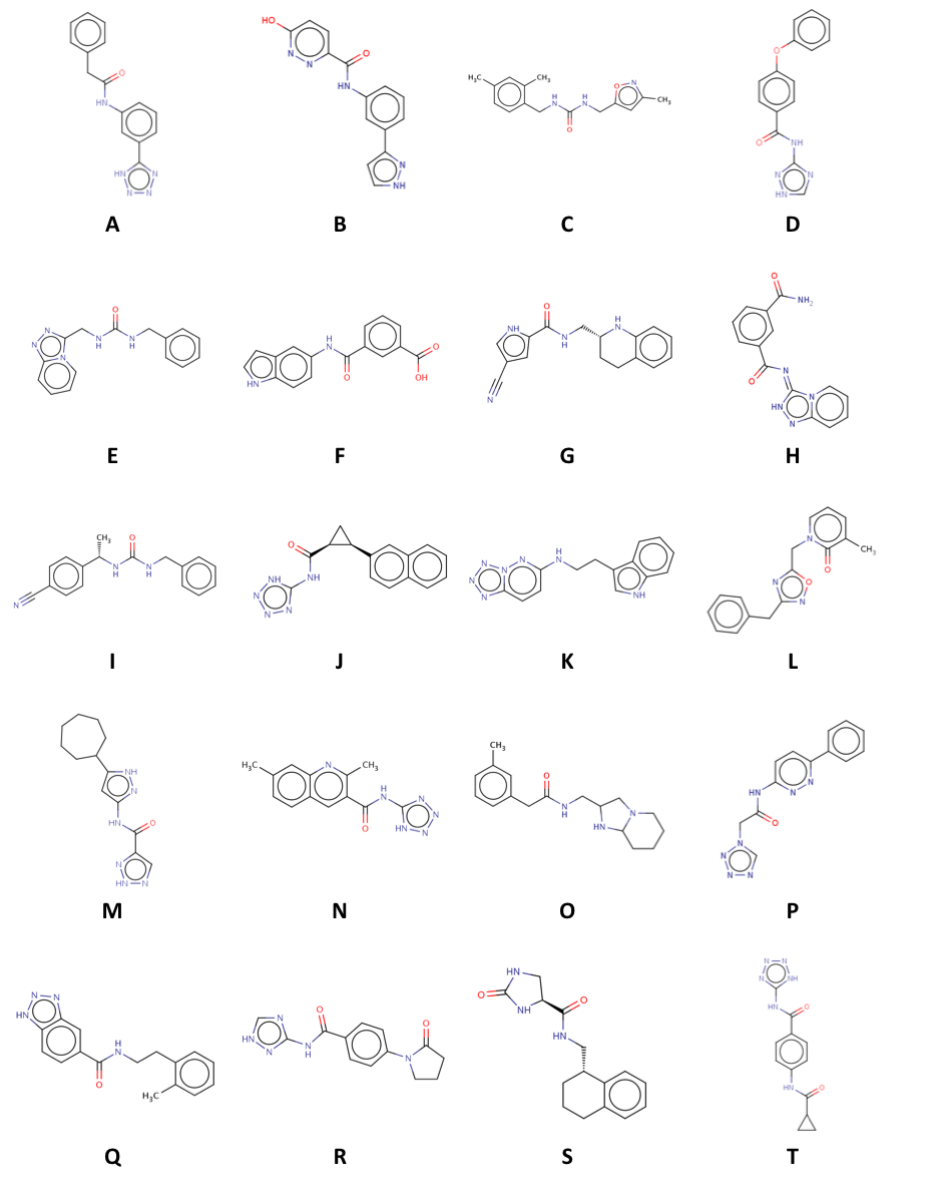
\includegraphics[width=\textwidth]{images/compound_structures}

\caption{Chemical structures of selected compounds to screen experimentally against a potential allosteric site on CDK2.
The compounds are labelled as in Table~\ref{tab:enamine_compounds}.}

\label{fig:compound_structures}
\end{figure}


\subsection{Purification of cyclin A}

Initially the purification of GST-tagged cyclin A was attempted.
This resulted in low quantities of soluble protein (x mg from y L culture) and purity was low.
The purification of His-tagged cyclin A however produced considerably more protein (x mg from y L culture), so it was decided to use this.
Fig with gel bands and different conditions.


\subsection{Binding assay}


\subsection{TR-FRET}


\section{Discussion}

Difficulty of purifying cyclin A, due to flexible structure?, also GST may affect folding, ref to lack of crystal structure for certain region (run Disopred to check disorder?).
